\typeout{************************************************}
\typeout{Chapter 12 Back to the Real Numbers}
\typeout{************************************************}
%
\begin{chapterptx}{Back to the Real Numbers}{}{Back to the Real Numbers}{}{}{x:chapter:BackToFourier}
	\begin{introduction}{}%
		As we have seen, when they converge, power series are very well behaved and Fourier (trigonometric) series are not necessarily. The fact that trigonometric series were so interesting made them a lightning rod for mathematical study in the late nineteenth century.%
		\par
		For example, consider the question of uniqueness. We saw in \hyperref[x:chapter:TaylorSeries]{Chapter~{\xreffont\ref{x:chapter:TaylorSeries}}} that if a function could be represented by a power series, then that series must be the Taylor series. More precisely, if%
		\begin{equation*}
			f(x)=\sum_{n=0}^\infty a_n(x-a)^n, \text{  then  }  a_n=\frac{f^{(n)}(a)}{n!}\text{.}
		\end{equation*}
		%
		\par
		But what can be said about the uniqueness of a trigonometric series? If we can represent a function \(f\) as a general trigonometric series%
		\begin{equation*}
			f(x)=\sum_{n=0}^\infty(a_n\cos n\pi x\,+b_n\sin n\pi x)\text{,}
		\end{equation*}
		then must this be the Fourier series with the coefficients as determined by Fourier? \index{Fourier, Jean Baptiste Joseph}%
		\par
		For example, if \(\sum_{n=0}^\infty(a_n\cos n\pi x\,+b_n\sin n\pi x)\) converges to \(f\) uniformly on the interval \((0,1)\), then because of the uniform convergence, Fourier's term-by-term integration which we saw in \hyperref[x:part:Interregnum]{Part~{\xreffont\ref{x:part:Interregnum}}} is perfectly legitimate and the coefficients are, of necessity, the coefficients he computed. However we have seen that the convergence of a Fourier series need not be uniform. This does not mean that we cannot integrate term-by-term, but it does say that we can't be sure that term-by-term integration of a Fourier series will yield the integral of the associated function.%
		\par
		\index{Lebesgue, Henri}\index{Cantor, Georg} This led to a generalization of the integral by Henri Lebesgue in 1905.  Lebesgue's profound work settled the issue of whether or not a bounded pointwise converging trigonometric series is the Fourier series of a function, but we will not go in this direction.  We will instead focus on work that Georg Cantor did in the years just prior. Cantor's work was also profound and had far reaching implications in modern mathematics.  It also leads to some very weird conclusions.%
		\begin{aside}{}{g:aside:idp328}%
			'Weird' does not mean false.  It simply means that some of Cantor's results can be hard to accept, even after you have seen the proof and verified its validity.%
		\end{aside}
		To begin, let's suppress the underlying function and suppose we have%
		\begin{equation*}
			\sum_{n=0}^\infty(a_n\cos n\pi x\,+b_n\sin n\pi x) = \sum_{n=0}^\infty(a^\prime_n\cos n\pi x\,+b^\prime_n\sin n\pi x)\text{.}
		\end{equation*}
		%
		\par
		We ask: If these two series are equal must it be true that \(a_n=a^\prime_n\) and \(b_n=b^\prime_n?\) We can reformulate this uniqueness question as follows: Suppose%
		\begin{equation*}
			\sum_{n=0}^\infty\left((a_n-a^\prime_n)\cos n\pi x\,+(b_n-b^\prime_n)\sin n\pi x\right) = 0\text{.}
		\end{equation*}
		%
		\par
		If we let \(c_n = a_n-a^\prime_n\) and \(d_n = b_n-b^\prime_n\), then the question becomes: If \(\sum_{n=0}^\infty\left(c_n\cos n\pi x\,+d_n\sin n\pi x\right) = 0\), then will \(c_n=d_n=0?\) It certainly seems reasonable to suppose so, but at this point we have enough experience with infinite sums to know that we need to be \emph{very} careful about relying on the intuition we have honed on finite sums.%
		\par
		\index{Cantor, Georg!and the modern view of mathematics} The answer to this seemingly basic question leads to some very profound results.  In particular, answering this question led the mathematician Georg Cantor (1845-1918) to study the makeup of the real number system.  This in turn opened the door to the modern view of mathematics of the twentieth century.  In particular, Cantor proved the following result in 1871~(\hyperlink{x:biblio:jahnke03__histor_analy}{[{\xreffont 6}]}, p. 305).%
		\begin{theorem}{}{}{x:theorem:thm_Cantor-uniqueness-of-trig-series}%
			\alert{Cantor}%
			\par
			\index{Cantor, Georg}\index{Cantor, Georg!uniqueness of Fourier series!first theorem on}\index{Fourier Series!Cantor's first theorem on uniqueness} If the trigonometric series%
			\begin{equation*}
				\sum_{n=0}^\infty\left(c_n\cos n\pi  x\,+d_n\sin n\pi x\right) = 0\text{,}
			\end{equation*}
			%
			\par
			``with the exception of certain values of \(x\),'' then all of its coefficients vanish.%
		\end{theorem}
		In his attempts to nail down precisely which ``certain values'' could be exceptional, Cantor was led to examine the nature of subsets of real numbers and ultimately to give a precise definition of the concept of infinite sets and to define an arithmetic of ``infinite numbers.'' (Actually, he called them \textbraceleft{}transfinite numbers\textbraceright{} because, by definition, numbers are finite.)%
		\par
		As a first step toward identifying those ``certain values,'' Cantor proved the following theorem, which we will state but not prove.%
		\begin{theorem}{}{}{x:theorem:thm_Cantor_1870}%
			\alert{Cantor, (1870)}%
			\par
			\index{Cantor, Georg!uniqueness of Fourier series!second theorem}\index{Fourier Series!Cantor's second theorem on uniqueness} If the trigonometric series%
			\begin{equation*}
				\sum_{n=0}^\infty\left(c_n\cos n\pi  x\,+d_n\sin n\pi x\right) = 0\text{,}
			\end{equation*}
			for all \(x\in\RR\) then all of its coefficients vanish.%
		\end{theorem}
		He then extended this to the following:%
		\begin{theorem}{}{}{x:theorem:thm_Cantor-1871-b}%
			\alert{Cantor, (1871)}%
			\par
			\index{Cantor, Georg!uniqueness of Fourier series!third theorem on}\index{Fourier Series!Cantor's third theorem on uniqueness} If the trigonometric series%
			\begin{equation*}
				\sum_{n=0}^\infty\left(c_n\cos n\pi  x\,+d_n\sin n\pi x\right) = 0\text{,}
			\end{equation*}
			for all but finitely many \(x\in\RR\) then all of its coefficients vanish.%
		\end{theorem}
		\begin{figureptx}{\href{https://mathshistory.st-andrews.ac.uk/Biographies/Cantor/}{Georg Cantor}\protect\footnotemark{}}{g:figure:idp329}{}%
			\index{Cantor, Georg!portrait of}%
			\begin{image}{0.325}{0.35}{0.325}%
				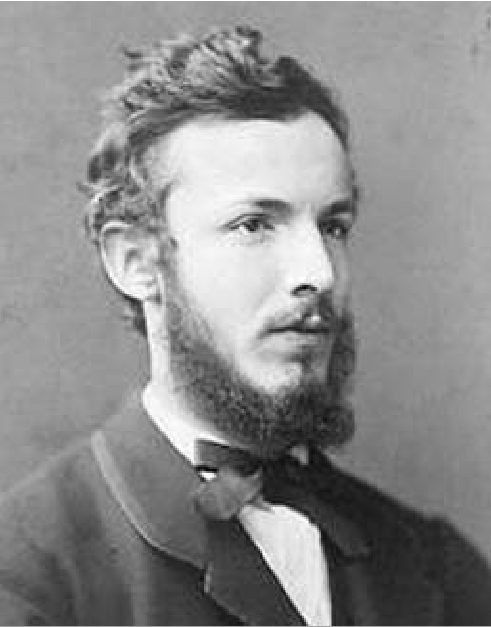
\includegraphics[width=\linewidth]{external/images/Cantor.png}
			\end{image}%
			\tcblower
		\end{figureptx}%
		\footnotetext[18]{\nolinkurl{mathshistory.st-andrews.ac.uk/Biographies/Cantor/}\label{g:fn:idp330}}%
		Observe that this is not a trivial generalization. Although the exceptional points are constrained to be finite in number, this number could still be extraordinarily large. That is, even if the series given above differed from zero on \(10^{10^{100000}}\) distinct points in the interval \((0, 10^{10^{-100000}})\) the coefficients still vanish. This remains true even if at each of these \(10^{10^{100000}}\) points the series converges to \(10^{10^{100000}}\). This is truly remarkable when you think of it this way.%
		\par
		At this point Cantor became more interested in these exceptional points than in the Fourier series problem that he'd started with. The next task he set for himself was to see just how general the set of exceptional points could be. Following Cantor's lead we make the following definitions.%
		\begin{definition}{}{x:definition:def_accumulation-point}%
			\index{limit!accumulation points}\index{sets!accumulation points} Let \(S\subseteq \RR\) and let \(a\) be a real number. We say that \(a\) is a \terminology{limit point} (or an \terminology{accumulation point}) of \(S\) if there is a sequence \((a_n)\) with \(a_n\in S-\left\{a\right\}\) which converges to \(a\).%
		\end{definition}
		\begin{problem}{}{g:problem:idp331}%
			\index{limit!accumulation point}\index{sets!accumulation points} Let \(S\subseteq\RR\) and let \(a\) be a real number. Prove that \(a\) is a limit point of \(S\) if and only if for every \(\eps>0\) the intersection%
			\begin{equation*}
				(a-\eps, a+\eps) \cap S-\left\{a\right\} \neq \emptyset.{}
			\end{equation*}
			%
		\end{problem}
		The following definition gets to the heart of the matter.%
		\begin{definition}{}{x:definition:def_derived-set}%
			\index{sets!derived sets} Let \(S\subseteq\RR\). The set of all limit points of \(S\) is called the \terminology{derived set} of \(S\). The derived set is denoted \(S^{\prime}\).%
		\end{definition}
		Don't confuse the derived set of a set with the derivative of a function. They are completely different objects despite the similarity of both the language and notation. The only thing that they have in common is that they were somehow ``derived'' from something else.%
		\begin{problem}{}{g:problem:idp332}%
			Determine the derived set, \(S^\prime\), of each of the following sets.%
			\begin{enumerate}[label=(\alph*)]
				\item{}\(\displaystyle S=\left\{\frac11, \frac12, \frac13, \ldots\right\}\)%
				\item{}\(\displaystyle S=\left\{0,\frac11, \frac12, \frac13, \ldots\right\}\)%
				\item{}\(\displaystyle S=(0,1]\)%
				\item{}\(\displaystyle S=\left[\left.0,1/2\right)\right.\cup\left.\left(1/2,1\right.\right]\)%
				\item{}\(\displaystyle S=\QQ\)%
				\item{}\(\displaystyle S=\RR-\QQ\)%
				\item{}\(\displaystyle S=\ZZ\)%
				\item{}Any finite set \(S\).%
			\end{enumerate}
			%
		\end{problem}
		\begin{problem}{}{g:problem:idp333}%
			\index{derived sets} Let \(S\subseteq\RR\).%
			\begin{enumerate}[label=(\alph*)]
				\item{}Prove that \(\left(S^{\,\prime}\right)^{\,\prime}\subseteq S^{\,\prime}\).%
				\item{}Give an example where these two sets are equal.%
				\item{}Give an example where these two sets are not equal.%
			\end{enumerate}
			%
		\end{problem}
		The notion of the derived set forms the foundation of Cantor's exceptional set of values. Specifically, let \(S\) again be a set of real numbers and consider the following sequence of sets:%
		\begin{equation*}
			S^{\,\prime}\supseteq \left(S^\prime\right)^\prime\supseteq \left(\left(S^\prime\right)^\prime\right)^\prime\supseteq \cdots\text{.}
		\end{equation*}
		%
		\par
		Cantor \index{Cantor, Georg} showed that if, at some point, one of these derived sets is empty, then the uniqueness property still holds. Specifically, we have:%
		\begin{theorem}{}{}{x:theorem:thm_Cantor-1871}%
			\alert{Cantor, (1871)}%
			\par
			\index{Cantor, Georg!fourth theorem on the uniqueness of Fourier series} Let \(S\) be a subset of the real numbers with the property that one of its derived sets is empty.  Then if the trigonometric series \(\sum_{n=0}^\infty\left(c_n\cos n\pi
			x\,+d_n\sin n\pi x\right)\) is zero for all \(x\in\RR-S\), then all of the coefficients of the series vanish.%
		\end{theorem}
	\end{introduction}%
	%
	%
	\typeout{************************************************}
	\typeout{Section 12.1 Infinite Sets}
	\typeout{************************************************}
	%
	\begin{sectionptx}{Infinite Sets}{}{Infinite Sets}{}{}{x:section:BackToFourier-InfiniteSets}
		The following theorem follows directly from our previous work with the NIP and will be very handy later. It basically says that a sequence of nested closed intervals will still have a non-empty intersection even if their lengths do not converge to zero as in the NIP.%
		\begin{theorem}{}{}{x:theorem:thm_WeakNIP}%
			\index{Nested Interval Property (NIP)!weak form} Let \(\left(\left[a_n, b_n\right]\right)_{n=1}^\infty\) be a sequence of nested intervals such that \(\limit{n}{\infty}{\abs{b_n-a_n}}>0\). Then there is at least one \(c\in\RR\) such that \(c\in\left[a_n, b_n\right]\) for all \(n\in\NN\).%
		\end{theorem}
		\begin{proof}{}{g:proof:idp334}
			By \hyperref[x:corollary:cor_IncBoundedConverge]{Corollary~{\xreffont\ref{x:corollary:cor_IncBoundedConverge}}} of \hyperref[x:chapter:IVTandEVT]{Chapter~{\xreffont\ref{x:chapter:IVTandEVT}}}, we know that a bounded increasing sequence such as \((a_n)\) converges, say to \(c\). Since \(a_n\leq a_m\leq b_n\) for \(m>n\) and \(\limit{m}{\infty}{a_m}=c\), then for any fixed \(n\), \(a_n\leq c\leq b_n\). This says \(c\in\left[a_n, b_n\right]\) for all \(n\in\NN\).%
		\end{proof}
		\begin{problem}{}{g:problem:idp335}%
			\index{Nested Interval Property (NIP)!weak form} Suppose \(\limit{n}{\infty}{\abs{b_n-a_n}}>0\).  Show that there are at least two points, \(c\) and \(d\), such that \(c\in[a_n, b_n]\) and \(d\in[a_n, b_n]\) for all \(n\in\NN\).%
		\end{problem}
		Our next theorem says that in a certain, very technical sense there are more real numbers than there are counting numbers \hyperlink{x:biblio:franks10__cantor_other_proof_rr_uncoun}{[{\xreffont 3}]}. This probably does not seem terribly significant.  After all, there are real numbers which are not counting numbers.  What will make this so startling is that the same cannot be said about all sets which strictly contain the counting numbers.  We will get into the details of this after the theorem is proved.%
		\begin{theorem}{}{}{x:theorem:thm_NoSeriesContainsAllReals}%
			\alert{Cantor, (1874)}%
			\par
			\index{Cantor, Georg!first proof that \(\RR\) is uncountable}\index{\(\RR\)!is uncountable!Cantor's first proof} Let \(S=\left(s_n\right)_{n=1}^\infty\) be a sequence of real numbers.  There is a real number \(c\), which is not in  \(S\).%
			\begin{aside}{}{g:aside:idp336}%
				To streamline things, we are abusing notation here as we are letting \(S\) denote both the sequence (which is ordered) and the underlying (unordered) set of entries in the sequence.%
			\end{aside}
		\end{theorem}
		\begin{proof}{}{g:proof:idp337}
			For the sake of obtaining a contradiction assume that the sequence \(S\) contains every real number; that is, \(S=\RR\). As usual we will build a sequence of nested intervals \(\left(\left[x_i, y_i\right]\right)_{i=1}^\infty\).%
			\par
			Let \(x_1\) be the smaller of the first two distinct elements of \(S\), let \(y_1\) be the larger and take \(\left[x_1,y_1\right]\) to be the first interval.%
			\par
			Next we assume that \(\left[x_{n-1}, y_{n-1}\right]\) has been constructed and build \(\left[x_n, y_n\right]\) as follows. Observe that there are infinitely many elements of \(S\) in \(\left(x_{n-1}, y_{n-1}\right)\) since \(S=\RR\). Let \(s_m\) and \(s_k\) be the \emph{first} two distinct elements of \(S\) such that%
			\begin{equation*}
				s_m, s_k \in \left(x_{n-1}, y_{n-1}\right) \text{.}
			\end{equation*}
			%
			\par
			Take \(x_n\) to be the smaller and \(y_n\) to be the larger of \(s_m\) and \(s_k\). Then \(\left[x_n, y_n\right]\) is the \(n\)th interval.%
			\par
			From the way we constructed them it is clear that%
			\begin{equation*}
				\left[x_1, y_1\right] \supseteq \left[x_2, y_2\right] \supseteq \left[x_3, y_3\right] \supseteq \ldots\text{.}
			\end{equation*}
			%
			\par
			Therefore by \hyperref[x:theorem:thm_WeakNIP]{Theorem~{\xreffont\ref{x:theorem:thm_WeakNIP}}} there is a real number, say \(c\), such that%
			\begin{equation*}
				c\in\left[x_n, y_n\right] \text{ for all }  n\in\NN\text{.}
			\end{equation*}
			%
			\par
			In fact, since \(x_1\lt x_2\lt x_3\ldots\lt y_3\lt y_2\lt y_1\) it is clear that%
			\begin{equation}
				x_n\lt c\lt y_n, \ \forall n\text{.}\label{x:men:eq_NIP-interval}
			\end{equation}
			%
			\par
			We will show that \(c\) is the number we seek. That the inequalities in \hyperref[x:men:eq_NIP-interval]{formula~({\xreffont\ref{x:men:eq_NIP-interval}})} are strict will play a crucial role.%
			\par
			To see that \(c\not\in S\) we suppose that \(c\in S\) and derive a contradiction.%
			\par
			So, suppose that \(c=s_p\) for some \(p\in\NN\). Then only \(\left\{s_1, s_2,\ldots,
			s_{p-1}\right\}\) appear before \(s_p\) in the sequence \(S\). Since each \(x_n\) is taken from \(S\) it follows that only finitely many elements of the sequence \((x_n)\) appear before \(s_p=c\) in the sequence as well.%
			\par
			Let \(x_l\) be the \emph{last} element of \((x_n)\) which appears before \(c=s_p\) in the sequence and consider \(x_{l+1}\). The way it was constructed, \(x_{l+1}\) was one of the first two distinct terms in the sequence \(S\) strictly between \(x_l\) and \(y_l\), the other being \(y_{l+1}\). Since \(x_{l+1}\) does not appear before \(c=s_p\) in the sequence and \(x_l\lt c\lt y_l\), it follows that either \(c=x_{l+1}\) or \(c=y_{l+1}\). However, this gives us a contradiction as we know from \hyperref[x:men:eq_NIP-interval]{formula~({\xreffont\ref{x:men:eq_NIP-interval}})} that \(x_{l+1}\lt c\lt y_{l+1}\).%
			\par
			Thus \(c\) is not an element of \(S\).%
		\end{proof}
		So how does this theorem show that there are ``more'' real numbers than counting numbers? Before we address that question we need to be very careful about the meaning of the word 'more' when we're talking about infinite sets.%
		\par
		First let's consider two finite sets, say \(A=\left\{\alpha,\beta,\gamma,\delta\right\}\) and \(B=\left\{a,b,c,d,e\right\}\). How do we know that \(B\) is the bigger set? (It obviously is.) Clearly we can just count the number of elements in both \(A\) and \(B\). Since \(\abs{A}=4\) and \(\abs{B}=5\) and \(4\lt 5\) \(B\) is clearly bigger. But we're looking for a way to determine the relative size of two sets without counting them because we have no way of counting the number of elements of an infinite set. Indeed, it isn't even clear what the phrase ``the number of elements'' might \emph{mean} when applied to the elements of an infinite set.%
		\par
		When we count the number of elements in a finite set what we're really doing is matching up the elements of the set with a set of consecutive positive integers, starting at \(1\). Thus since%
		\begin{align*}
			1\amp \leftrightarrow\alpha\\
			2\amp \leftrightarrow\beta\\
			3\amp \leftrightarrow\gamma\\
			4\amp \leftrightarrow\delta
		\end{align*}
		we see that \(\abs{A}=4\). Moreover, the order of the match-up is unimportant. Thus since%
		\begin{align*}
			2\amp \leftrightarrow e\\
			3\amp \leftrightarrow a\\
			5\amp \leftrightarrow b\\
			4\amp \leftrightarrow d\\
			1\amp \leftrightarrow c
		\end{align*}
		it is clear that the elements of \(B\) and the set \(\left\{1,2,3,4,5\right\}\) can be matched up as well. And it doesn't matter what order either set is in. They both have \(5\) elements.%
		\par
		Such a match-up is called a one-to-one correspondence. In general, if two sets can be put in one-to-one correspondence then they are the same ``size.'' Of course the word ``size'' has lots of connotations that will begin to get in the way when we talk about infinite sets, so instead we will say that the two sets have the same \emph{cardinality.} Speaking loosely, this just means that they are the same size.%
		\par
		More precisely, if a given set \(S\) can be put in one-to-one correspondence with a finite set of consecutive integers, say \(\left\{1,2,3,\ldots, N\right\}\), then we say that the cardinality of the set is \(N\). But this just means that both sets have the same cardinality. It is this notion of one-to-one correspondence, along with the next two definitions, which will allow us to compare the sizes (cardinalities) of infinite sets.%
		\begin{definition}{}{x:definition:def_CountableSets}%
			\index{cardinality!countable sets}\index{countable sets!defintion of} Any set which can be put into one-to-one correspondence with \(\NN=\left\{1,2,3,\ldots\right\}\) is called a \terminology{countably infinite} set. Any set which is either finite or countably infinite is said to be \terminology{countable}.%
		\end{definition}
		Since \(\NN\) is an infinite set, we have no symbol to designate its cardinality so we have to invent one. The symbol used by Cantor \index{Cantor, Georg} and adopted by mathematicians ever since is \(\aleph_0\). Thus the cardinality of any countably infinite set is \(\aleph_0\).%
		\begin{aside}{}{g:aside:idp338}%
			\(\aleph{}\) is the first letter of the Hebrew alphabet and is pronounced "aleph." \(\aleph_0\) is pronounced "aleph null."%
		\end{aside}
		We have already given the following definition informally. We include it formally here for later reference.%
		\begin{definition}{}{x:definition:def_EqualCardinality}%
			\index{cardinality!equal cardinality} If two sets can be put into one-to-one correspondence then they are said to have the \alert{same cardinality}.%
		\end{definition}
		With these two definitions in place we can see that \hyperref[x:theorem:thm_NoSeriesContainsAllReals]{Theorem~{\xreffont\ref{x:theorem:thm_NoSeriesContainsAllReals}}} is nothing less than the statement that the real numbers are not countably infinite. Since it is certainly not finite, then we say that the set of real numbers is uncountable and therefore ``bigger'' than the natural numbers!%
		\par
		To see this let us suppose first that each real number appears in the sequence \((s_n)_{n=1}^\infty\) exactly once. In that case the indexing of our sequence is really just a one-to-one correspondence between the elements of the sequence and \(\NN:\)%
		\begin{align*}
			1\amp \leftrightarrow s_1\\
			2\amp \leftrightarrow s_2\\
			3\amp \leftrightarrow s_3\\
			4\amp \leftrightarrow s_4\\
			\amp \ \ \ \vdots
		\end{align*}
		%
		\par
		If some real numbers are repeated in our sequence then all of the real numbers are a subset of our sequence and will therefore also be countable (see \hyperref[x:problem:prob_countable_sets_unions_of]{Problem~{\xreffont\ref{x:problem:prob_countable_sets_unions_of}}}, part a).%
		\par
		In either case, every sequence is countable. But our theorem says that \emph{no} sequence in \(\RR\) includes all of \(\RR\). Therefore \(\RR\) is uncountable.%
		\par
		Most of the sets you have encountered so far in your life have been countable.%
		\begin{problem}{}{g:problem:idp339}%
			Show that each of the following sets is countable.%
			\begin{enumerate}[font=\bfseries,label=(\alph*),ref=\alph*]
				\item{}\(\left\{2,3,4,5,\ldots\right\}=\left\{n\right\}_{n=2}^\infty\)%
				\item{}\(\left\{0,1,2,3,\ldots\right\}=\left\{n\right\}_{n=0}^\infty\)%
				\item{}\(\left\{1,4,9,16,\ldots,n^2,\ldots\right\}=\left\{n^2\right\}_{n=1}^\infty\)%
				\item{}The set of prime numbers%
				\item{}\(\ZZ\)%
			\end{enumerate}
		\end{problem}
		In fact, if we start with a countable set it is rather difficult to use it to build anything but another countable set.%
		\begin{problem}{}{x:problem:prob_countable_sets_unions_of}%
			Let \(\left\{A_i\right\}\) be a collection of countable sets. Show that each of the following sets is also countable:%
			\begin{enumerate}[font=\bfseries,label=(\alph*),ref=\alph*]
				\item{}Any subset of \(A_1\).%
				\item{}\(A_1\cup A_2\)%
				\item{}\(A_1\cup A_2 \cup A_3\)%
				\item{}\(\displaystyle\bigcup_{i=1}^nA_i\)%
				\item{}\(\displaystyle\bigcup_{i=1}^\infty A_i\)%
			\end{enumerate}
		\end{problem}
		It seems that no matter what we do the only example of an uncountably infinite set is \(\RR\).  But wait!  Remember the rational numbers?  They were similar to the real numbers in many ways.  Perhaps they are uncountably infinite too?%
		\par
		Alas, no. The rational numbers turn out to be countable too.%
		\begin{theorem}{}{}{x:theorem:thm_QisCountable}%
			\index{\(\QQ\)!is countable} Show that \(\QQ\) is countable.%
		\end{theorem}
		\begin{proof}{Sketch of Proof.}{g:proof:idp340}
			First explain how you know that all of the non-negative rational numbers are in this list:%
			\begin{equation*}
				\frac{0}{1},\frac{0}{2},\frac{1}{1},\frac{0}{3}, \frac{1}{2},\frac{2}{1},\frac{0}{4},\frac{1}{3}, \frac{2}{2}, \frac{3}{1}, \cdots\text{.}
			\end{equation*}
			%
			\par
			However there is clearly some duplication. To handle this, apply part (a) of \hyperref[x:problem:prob_countable_sets_unions_of]{Problem~{\xreffont\ref{x:problem:prob_countable_sets_unions_of}}}. Does this complete the proof or is there more to do?%
		\end{proof}
		\begin{problem}{}{g:problem:idp341}%
			\index{\(\QQ\)!\(\QQ\) is countable} Prove \hyperref[x:theorem:thm_QisCountable]{Theorem~{\xreffont\ref{x:theorem:thm_QisCountable}}}.%
		\end{problem}
		The following corollary says that the cardinality of the real numbers is \emph{much} larger than the cardinality of the rational numbers, despite the fact that both are infinite.%
		\par
		That is, as a subset of the reals, the rationals can be contained in a sequence of intervals, the sum of whose lengths can be arbitrarily small. In a sense this says that a countably infinite set is so small (on the transfinite scale) that it is ``almost'' finite.%
		\par
		\index{measure zero} Usually we express this idea with the statement, ``\(\QQ\) is a set of \emph{measure zero} in \(\RR\)''. The term ``measure'' has a precise meaning which we will not pursue. The following corollary contains the essence of the idea.%
		\begin{corollary}{}{}{x:corollary:cor_Q-MeasureZero}%
			Let \(\eps>0\) be given. There is a collection of intervals in \(\RR\), \(I_n=[a_n,b_n]\) such that%
			\begin{equation*}
				\QQ \subset \bigcup_{n=1}^\infty I_n
			\end{equation*}
			and%
			\begin{equation*}
				\sum_{n=1}^\infty(b_n-a_n)\lt \eps\text{.}
			\end{equation*}
			%
		\end{corollary}
		\begin{problem}{}{g:problem:idp342}%
			\index{\(\QQ\)!has measure zero in \(\RR\)}\index{measure zero!\(\QQ\) has measure zero in \(\RR\)} Prove \hyperref[x:corollary:cor_Q-MeasureZero]{Corollary~{\xreffont\ref{x:corollary:cor_Q-MeasureZero}}}.%
			\par\smallskip%
			\noindent\textbf{\blocktitlefont Hint}.\hypertarget{g:hint:idp343}{}\quad{}If we had only finitely many rationals to deal with this would be easy. Let \(\left\{r_1, r_2, \ldots,
			r_k\right\}\) be these rational numbers and take \(a_n=r_n-\frac{\eps}{2(k+1)}\) and \(b_n=r_n+\frac{\eps}{2(k+1)}\). Then for all \(n=1,\ldots, k\) \(r_n\in[a_n,b_n]\) and%
			\begin{equation*}
				\sum_{n=1}^kb_n-a_n = \sum_{n=1}^k \frac{\eps}{k+1}=\frac{k\eps}{k+1}\lt\eps\text{.}
			\end{equation*}
			%
			\par
			The difficulty is, how do we move from the finite to the infinite case?]%
		\end{problem}
		Notice how this idea hearkens back to the discussion of Leibniz's\index{Leibniz, Gottfried Wilhelm} approach to the Product Rule (\hyperref[x:men:eq_LeibnizProductRule]{equation~({\xreffont\ref{x:men:eq_LeibnizProductRule}})}). He simply tossed aside the expression \(\dx{ x}\dx{ y}\) because it was \emph{infinitely small} compared to either \(x\dx{ y}\) or \(y\dx{ x}\). Although this isn't quite the same thing we are discussing here it is similar and it is clear that Leibniz's insight and intuition were extremely acute. They were moving him in the right direction, at least.%
		\par
		All of our efforts to build an uncountable set from a countable one have come to nothing. In fact many sets that at first ``feel'' like they should be uncountable are in fact countable. This makes the uncountability of \(\RR\) all the more remarkable.%
		\begin{aside}{}{g:aside:idp344}%
			The failure is in the methods we've used so far.  It is possible to build an uncountable set using just two symbols if we're clever enough, but this would take us too far away from our main topic.%
		\end{aside}
		However if we \emph{start} with an uncountable set it is relatively easy to build others from it.%
		\begin{problem}{}{g:problem:idp345}%
			\begin{enumerate}[font=\bfseries,label=(\alph*),ref=\alph*]
				\item{}Let \((a,b)\) and \((c,d)\) be two open intervals of real numbers.  Show that these two sets have the same cardinality by constructing a one-to-one onto function between them.%
				\par\smallskip%
				\noindent\textbf{\blocktitlefont Hint}.\hypertarget{g:hint:idp346}{}\quad{}A linear function should do the trick.%
				\item{}Show that any open interval of real numbers has the same cardinality as \(\RR\).%
				\par\smallskip%
				\noindent\textbf{\blocktitlefont Hint}.\hypertarget{g:hint:idp347}{}\quad{}Consider the interval \((-\pi/2,\pi/2)\).%
				\item{}Show that \((0,1]\) and \((0,1)\) have the same cardinality.%
				\par\smallskip%
				\noindent\textbf{\blocktitlefont Hint}.\hypertarget{g:hint:idp348}{}\quad{}Note that \(\left\{1,1/2,1/3,\ldots\right\}\) and \(\left\{1/2, 1/3, \ldots\right\}\) have the same cardinality.%
				\item{}Show that \([0,1]\) and \((0,1)\) have the same cardinality.%
			\end{enumerate}
		\end{problem}
	\end{sectionptx}
	%
	%
	\typeout{************************************************}
	\typeout{Section 12.2 Cantor's Theorem and Its Consequences}
	\typeout{************************************************}
	%
	\begin{sectionptx}{Cantor's Theorem and Its Consequences}{}{Cantor's Theorem and Its Consequences}{}{}{x:section:BackToFourier-CantorsTheorem}
		\begin{figureptx}{\href{https://mathshistory.st-andrews.ac.uk/Biographies/Dedekind/}{Richard Dedekind}\protect\footnotemark{}}{g:figure:idp349}{}%
			\index{Dedekind, Richard!portrait of}%
			\begin{image}{0.325}{0.35}{0.325}%
				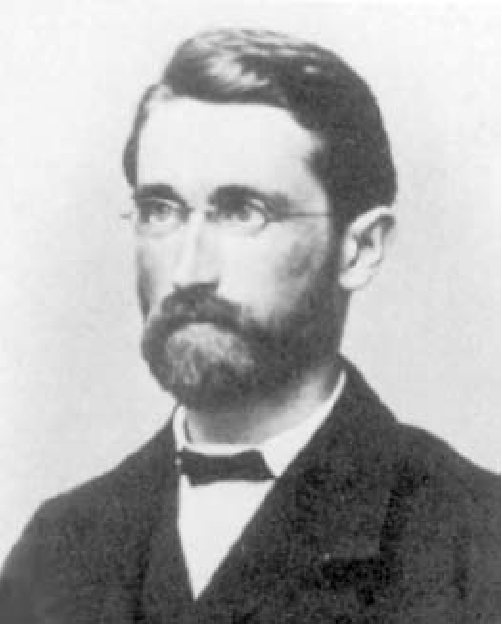
\includegraphics[width=\linewidth]{external/images/Dedekind.png}
			\end{image}%
			\tcblower
		\end{figureptx}%
		\footnotetext[19]{\nolinkurl{mathshistory.st-andrews.ac.uk/Biographies/Dedekind/}\label{g:fn:idp350}}%
		Once Cantor showed that there were two types of infinity (countable and uncountable), the following question was natural, ``Do all uncountable sets have the same cardinality?''%
		\par
		Just like not all ``non-dogs'' are cats, there is, offhand, no reason to believe that all uncountable sets should be the same size. However constructing uncountable sets of different sizes is not as easy as it sounds.%
		\par
		\index{Dedekind, Richard}\index{Cantor, Georg!unit interval and unit square have equal cardinalty} For example, what about the line segment represented by the interval \([0,1]\) and the square represented by the set \([0,1]\times[0,1]=\left\{(x,y)|0\leq x,y\leq 1\right\}\). Certainly the two dimensional square must be a larger infinite set than the one dimensional line segment.  Remarkably, Cantor showed that these two sets were the same cardinality.  In his 1877 correspondence of this result to his friend and fellow mathematician, Richard Dedekind, even Cantor remarked, ``I see it, but I don't believe it!''%
		\par
		The following gives the original idea of Cantor's proof. Cantor devised the following function \(f:[0,1]\times[0,1]\rightarrow [0,1]\). First, we represent the coordinates of any point \((x,y)\in [0,1]\times[0,1]\) by their decimal representations \(x=0.a_1 a_2 a_3\ldots\) and \(y=0.b_1 b_2 b_3\ldots\). Even terminating decimals can be written this way as we could write \(0.5=0.5000\ldots\). We can then define \(f(x,y)\) by%
		\begin{equation*}
			f((0.a_1 a_2 a_3\ldots ,0.b_1 b_2 b_3\ldots))=0.a_1 b_1 a_2 b_2 a_3 b_3\ldots\text{.}
		\end{equation*}
		%
		\par
		This relatively simple idea has some technical difficulties in it related to the following result.%
		\begin{problem}{}{g:problem:idp351}%
			\index{series!Geometric series!\((0.\bar{9})\) converges to \(1\)} Consider the sequence \((0.9,0.99,0.999,\ldots)\). Determine that this sequence converges and, in fact, it converges to \(1\). This suggests that \(0.999\ldots=1\).%
		\end{problem}
		Similarly, we have \(0.04999\ldots=0.05000\ldots\), etc. To make the decimal representation of a real number in \([0,1]\) unique, we must make a consistent choice of writing a terminating decimal as one that ends in an infinite string of zeros or an infinite string of nines [with the one exception \(0=0.000\ldots\) ]. No matter which choice we make, we could never make this function onto. For example, \(109/1100=0.09909090\ldots\) would have as its pre-image \((0.0999\ldots,0.9000\ldots)\) which would be a mix of the two conventions.%
		\par
		Cantor was able to overcome this technicality to demonstrate a one to one correspondence, but instead we will note that in either convention, the function is one-to-one, so this says that the set \([0,1]\times[0,1]\) is the same cardinality as some (uncountable) subset of \(\RR\).  The fact that this has the same cardinality as \(\RR\) is something we will come back to. But first we'll try construct an uncountable set which does not have the same cardinality as \(\RR\).  To address this issue, Cantor proved the following in 1891.%
		\begin{theorem}{}{}{x:theorem:thm_CantorsTheorem}%
			\alert{Cantor's Theorem}%
			\par
			\index{Cantor, Georg!Cantor's Theorem} Let \(S\) be any set.  Then there is no one-to-one correspondence between \(S\) and \(P(S)\), the set of all subsets of \(S\).%
		\end{theorem}
		Since \(S\) can be put into one-to-one correspondence with a subset of \(P(S)\) (\(a\rightarrow \left\{a\right\}\)), then this says that \(P(S)\) is at least as large as S. In the finite case \(\abs{P(S)}\) is strictly greater than \(\abs{S}\) as the following problem shows. It also demonstrates why \(P(S)\) is called the power set of \(S\).%
		\begin{problem}{}{x:problem:prob_PowerSet}%
			Prove: If \(\abs{S}=n\), then \(\abs{ P(S)}=2^n\).%
			\par\smallskip%
			\noindent\textbf{\blocktitlefont Hint}.\hypertarget{g:hint:idp352}{}\quad{}Let \(S=\left\{a_1,a_2,\ldots,a_n\right\}\). Consider the following correspondence between the elements of \(P(S)\) and the set \(T\) of all \(n\)-tuples of yes (Y) or no (N):%
			\begin{align*}
				\{ \}  \amp \leftrightarrow \{N,N,N,\ldots,N\}\\
				\{a_1\}\amp \leftrightarrow \{Y,N,N,\ldots ,N\}\\
				\{a_2\}\amp \leftrightarrow \{N,Y,N,\ldots,N\}\\
				\amp \vdots\\
				S\amp \leftrightarrow \{Y,Y,Y,\ldots,Y\}
			\end{align*}
			%
			\par
			How many elements are in \(T?\)%
		\end{problem}
		\begin{problem}{}{g:problem:idp353}%
			Prove \hyperref[x:theorem:thm_CantorsTheorem]{Cantor's Theorem~{\xreffont\ref{x:theorem:thm_CantorsTheorem}}}.%
			\par\smallskip%
			\noindent\textbf{\blocktitlefont Hint}.\hypertarget{g:hint:idp354}{}\quad{}Assume for contradiction, that there is a one-to-one correspondence \(f:S\rightarrow P(S)\). Consider \(A=\left\{x\in S|x\not\in f(x)\right\}\). Since \(f\) is onto, then there is \(a\in A\) such that \(A=f(a)\).  Is \(a\in A\) or is \(a\not\in
			A?\)%
		\end{problem}
		Actually it turns out that \(\RR\) and \(P(\NN)\) have the same cardinality. This can be seen in a roundabout way using some of the above ideas from \hyperref[x:problem:prob_PowerSet]{Problem~{\xreffont\ref{x:problem:prob_PowerSet}}}. Specifically, let \(T\) be the set of all sequences of zeros or ones (you can use \(Y\)s or \(N\)s, if you prefer). Then it is straightforward to see that \(T\) and \(P(\NN)\) have the same cardinality.%
		\par
		If we consider \((0,1]\), which has the same cardinality as \(\RR\), then we can see that this has the same cardinality as \(T\) as well. Specifically, if we think of the numbers in binary, then every real number in \([0,1]\) can be written as \(\sum_{j=1}^\infty \frac{a_j}{2^j} =0.a_1a_2a_3\ldots\) where \(a_j\in\left\{0,1\right\}\). We have to account for the fact that binary representations such as \(0.0111\ldots\) and \(0.1000\ldots\) represent the same real number (say that no representations will end in an infinite string of zeros), then we can see that \([0,1]\) has the same cardinality as \(T-U\), where \(U\) is the set of all sequences ending in an infinite string of zeros. It turns out that \(U\) itself is a countable set.%
		\begin{problem}{}{g:problem:idp355}%
			\index{countable sets!countable union of finite sets} Let \(U_n=\{(a_1,a_2,a_3,\ldots)\ |\ a_j\in \{0,1\} \text{ and } a_{n+1}=a_{n+2}=\cdots=0\}\). Show that for each \(n\), \(U_n\) is finite and use this to conclude that \(U\) is countably infinite.%
		\end{problem}
		The following two problems show that deleting a countable set from an uncountable set does not change its cardinality.%
		\begin{problem}{}{g:problem:idp356}%
			\index{sets!countably infinite subsets} Let \(S\) be an infinite set. Prove that \(S\) contains a countably infinite subset.%
		\end{problem}
		\begin{problem}{}{g:problem:idp357}%
			Suppose \(X\) is an uncountable set and \(Y\subset X\) is countably infinite.  Prove that \(X\) and \(X-Y\) have the same cardinality.%
			\par\smallskip%
			\noindent\textbf{\blocktitlefont Hint}.\hypertarget{g:hint:idp358}{}\quad{}Let \(Y=Y_0\). If \(X-Y_0\) is an infinite set, then by the previous problem it contains a countably infinite set \(Y_1\). Likewise if \(X-(Y_0\cup Y_1)\) is infinite it also contains an infinite set \(Y_2\). Again, if \(X-(Y_0\cup Y_1\cup Y_2)\) is an infinite set then it contains an infinite set \(Y_3\), etc. For \(n=1, 2, 3,\ldots \), let \(f_n:Y_{n-1}\rightarrow Y_n\) be a one-to-one correspondence and define \(f:X\rightarrow X-Y\) by%
			\begin{equation*}
				\begin{cases}f(x)=f_n(x), \amp \text{ if }  x\in Y_n, n=0,1,2,\ldots\\ f(x)=x, \amp \text{ if }  x\in X-(\cup_{n=0}^\infty Y_n ) \end{cases} \text{.}
			\end{equation*}
			%
			\par
			Show that \(f\) is one-to-one and onto.%
		\end{problem}
		The above problems say that \(R\), \(T-U\), \(T\), and \(P(N)\) all have the same cardinality.%
		\par
		As was indicated before, Cantor's \index{Cantor, Georg} work on infinite sets had a profound impact on mathematics in the beginning of the twentieth century. For example, in examining the proof of Cantor's Theorem, the eminent logician Bertrand Russell devised his famous paradox in 1901. Before this time, a set was naively thought of as just a collection of objects. Through the work of Cantor and others, sets were becoming a central object of study in mathematics as many mathematical concepts were being reformulated in terms of sets. The idea was that set theory was to be a unifying theme of mathematics. This paradox set the mathematical world on its ear.%
		\par
		\textbraceleft{}Russell's Paradox\textbraceright{} \index{Russell's Paradox} Consider the set of all sets which are not elements of themselves. We call this set \(D\) and ask, ``Is \(D\in D?\)'' Symbolically, this set is%
		\begin{equation*}
			D=\{S\ |\ S\not \in S\}\text{.}
		\end{equation*}
		%
		\par
		If \(D\in D\), then by definition, \(D\not\in D\). If \(D\not\in D\), then by definition, \(D\in D\).%
		\par
		If you look back at the proof of Cantor's Theorem, this was basically the idea that gave us the contradiction.  To have such a contradiction occurring at the most basic level of mathematics was scandalous.  It forced a number of mathematicians and logicians to carefully devise the axioms by which sets could be constructed. To be honest, most mathematicians still approach set theory from a naive point of view as the sets we typically deal with fall under the category of what we would call ``normal sets.'' In fact, such an approach is officially called Naive Set Theory (as opposed to Axiomatic Set Theory).  However, attempts to put set theory and logic on solid footing led to the modern study of symbolic logic and ultimately the design of computer (machine) logic.%
		\par
		Another place where Cantor's work had a profound influence in modern logic comes from something we alluded to before.  We showed before that the unit square \([0,1]\times [0,1]\) had the same cardinality as an uncountable subset of \(\RR\).  In fact, Cantor \index{Cantor, Georg} showed that the unit square had the same cardinality as \(\RR\) itself and was moved to advance the following in 1878.%
		\begin{conjecture}{The Continuum Hypothesis.}{}{g:conjecture:idp359}%
			\index{Continuum Hypothesis!original}%
			Every uncountable subset of \(\RR\) has the same cardinality as \(\RR\).%
		\end{conjecture}
		Cantor was unable to prove or disprove this conjecture (along with every other mathematician). In fact, proving or disproving this conjecture, which was dubbed the Continuum Hypothesis, was one of Hilbert's famous 23 problems presented as a challenge to mathematicians at the International Congress of Mathematicians in 1900.%
		\par
		Since \(\RR\) has the same cardinality as \(P(\NN)\), then the Continuum Hypothesis was generalized to the:%
		\begin{conjecture}{The Generalized Continuum Hypothesis.}{}{g:conjecture:idp360}%
			\index{Continuum Hypothesis!generalized}%
			Given an infinite set \(S\), there is no infinite set which has a cardinality strictly between that of \(S\) and its power set \(P(S)\).%
		\end{conjecture}
		\begin{aside}{The Zermelo-Fraenkel Axioms.}{g:aside:idp361}%
			One of the formal axiomatic approaches to set theory established by Ernst Zermelo in 1908 and revised by Abraham Fraenkel in 1921.%
		\end{aside}
		Efforts to prove or disprove this were in vain and with good reason.  In 1940, the logician Kurt Gödel showed that the Continuum Hypothesis could not be disproved from the Zermelo-Fraenkel Axioms of set theory.  In 1963, Paul Cohen showed that the Continuum Hypothesis could not be proved using the Zermelo-Fraenkel Axioms.  In other words, the Zermelo-Fraenkel Axioms do not contain enough information to decide the truth of the hypothesis.%
		\par
		We are willing to bet that at this point your head might be swimming a bit with uncertainty. If so, then know that these are the same feelings that the mathematical community experienced in the mid twentieth century. In the past, mathematics was seen as a model of logical certainty. It is disconcerting to find that there are statements that are ``undecidable.'' In fact, Gödel proved in 1931 that a consistent finite axiom system that contained the axioms of arithmetic would always contain undecidable statements which could neither be proved true nor false with those axioms. Mathematical knowledge would always be incomplete.%
		\begin{figureptx}{\href{https://mathshistory.st-andrews.ac.uk/Biographies/Godel/}{Kurt Gödel}\protect\footnotemark{}}{g:figure:idp362}{}%
			\index{Gödel, Kurt!portrait of}%
			\begin{image}{0.325}{0.35}{0.325}%
				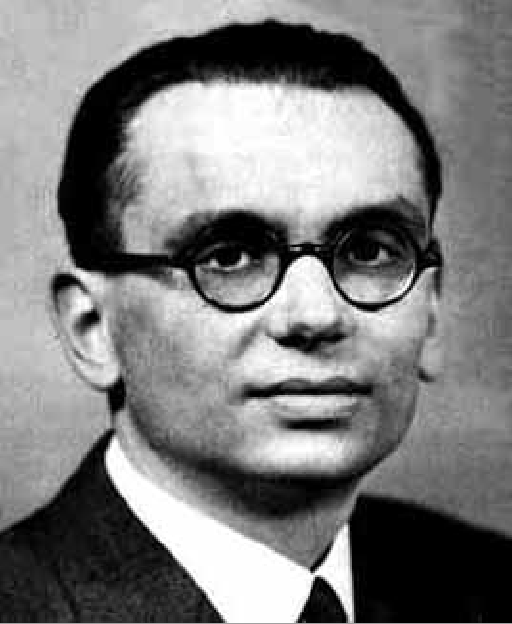
\includegraphics[width=\linewidth]{external/images/Godel.png}
			\end{image}%
			\tcblower
		\end{figureptx}%
		\footnotetext[20]{\nolinkurl{mathshistory.st-andrews.ac.uk/Biographies/Godel/}\label{g:fn:idp363}}%
		So by trying to put the foundations of calculus on solid ground, we have come to a point where we can never obtain mathematical certainty. Does this mean that we should throw up our hands and concede defeat? Should we be paralyzed with fear of trying anything? Certainly not! As we mentioned before, most mathematicians do well by taking a pragmatic approach: using their mathematics to solve problems that they encounter. In fact, it is typically the problems that motivate the mathematics. It is true that mathematicians take chances that don't always pan out, but they still take these chances, often with success. Even when the successes lead to more questions, as they typically do, tackling those questions usually leads to a deeper understanding. At the very least, our incomplete understanding means we will always have more questions to answer, more problems to solve.%
		\par
		What else could a mathematician ask for?%
	\end{sectionptx}
\end{chapterptx}
%
%